\begin{frame}{Candidate descriptor leaders: potential and capacity}
\centering
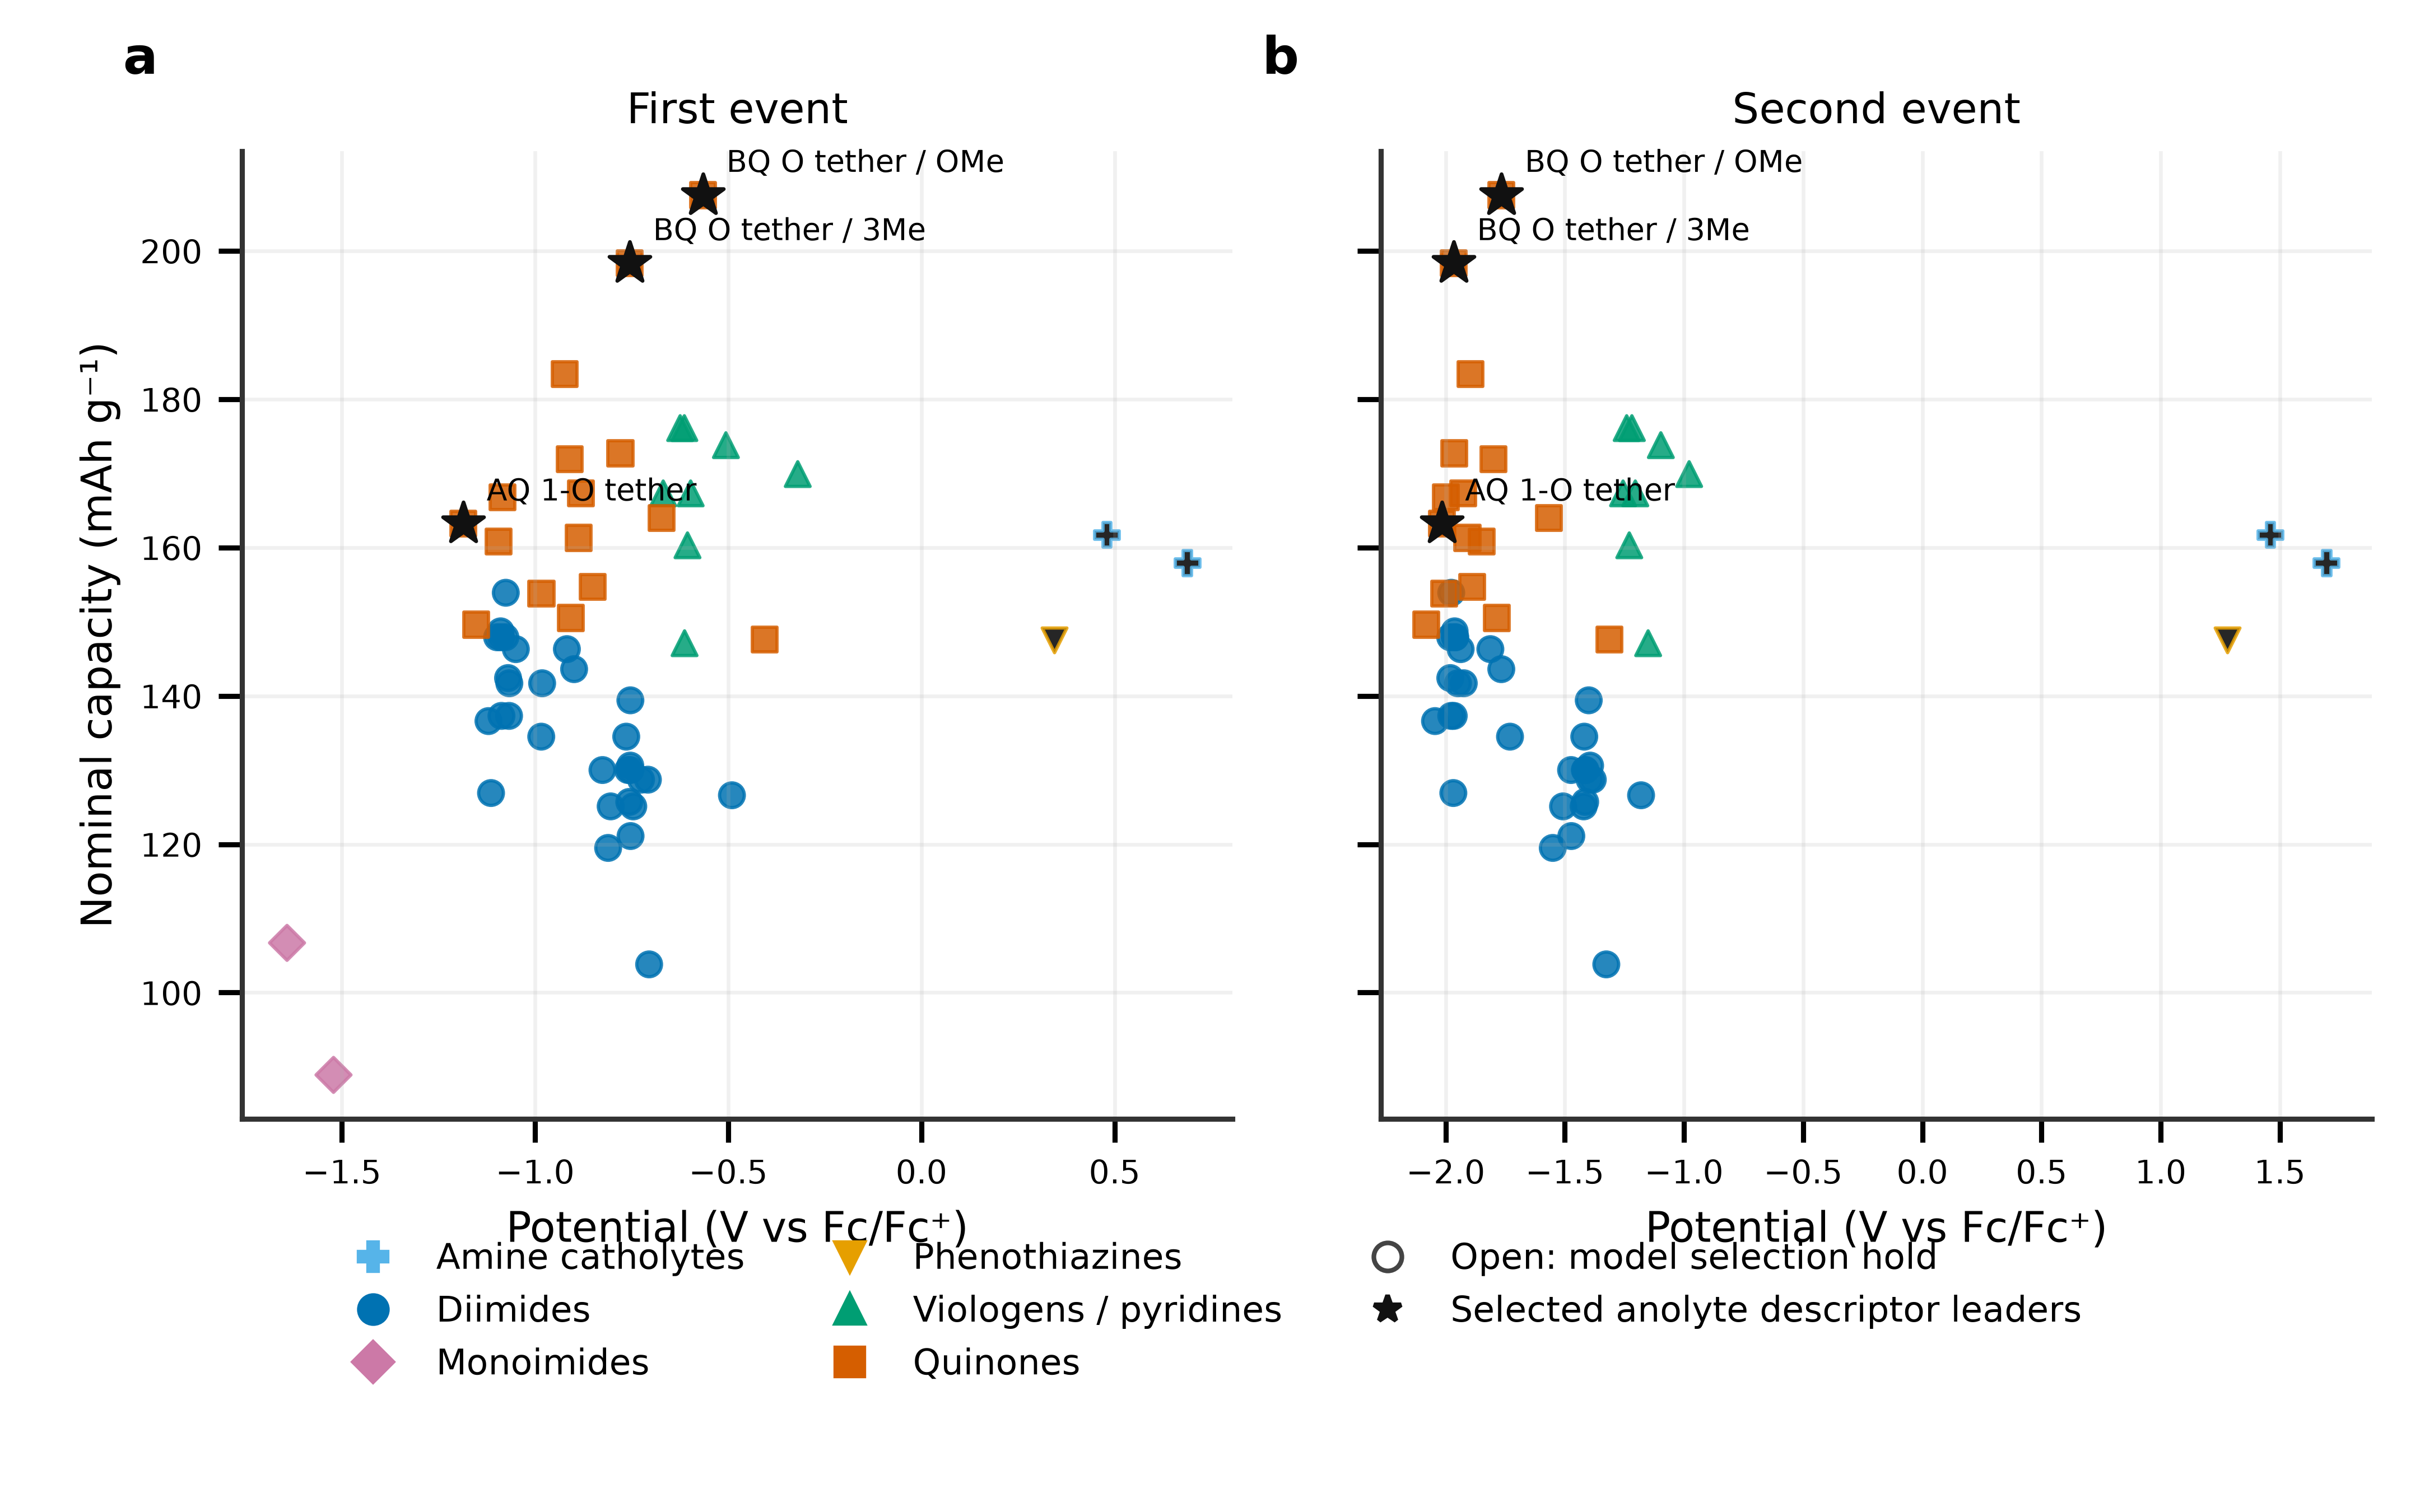
\includegraphics[width=.97\linewidth,height=.72\textheight,keepaspectratio]{../results/candidates/figures/redox_capacity.png}
\par\smallskip\raggedright\scriptsize Stars select anolyte descriptor leaders on a partial potential--capacity front. Kinetics and polymer validation remain pending.
\vfill\tiny Audited model snapshot: 2026-10-19T12:22:05.478576-05:00.
\end{frame}
\begin{frame}{Synthesis accessibility is a separate consideration}
\centering
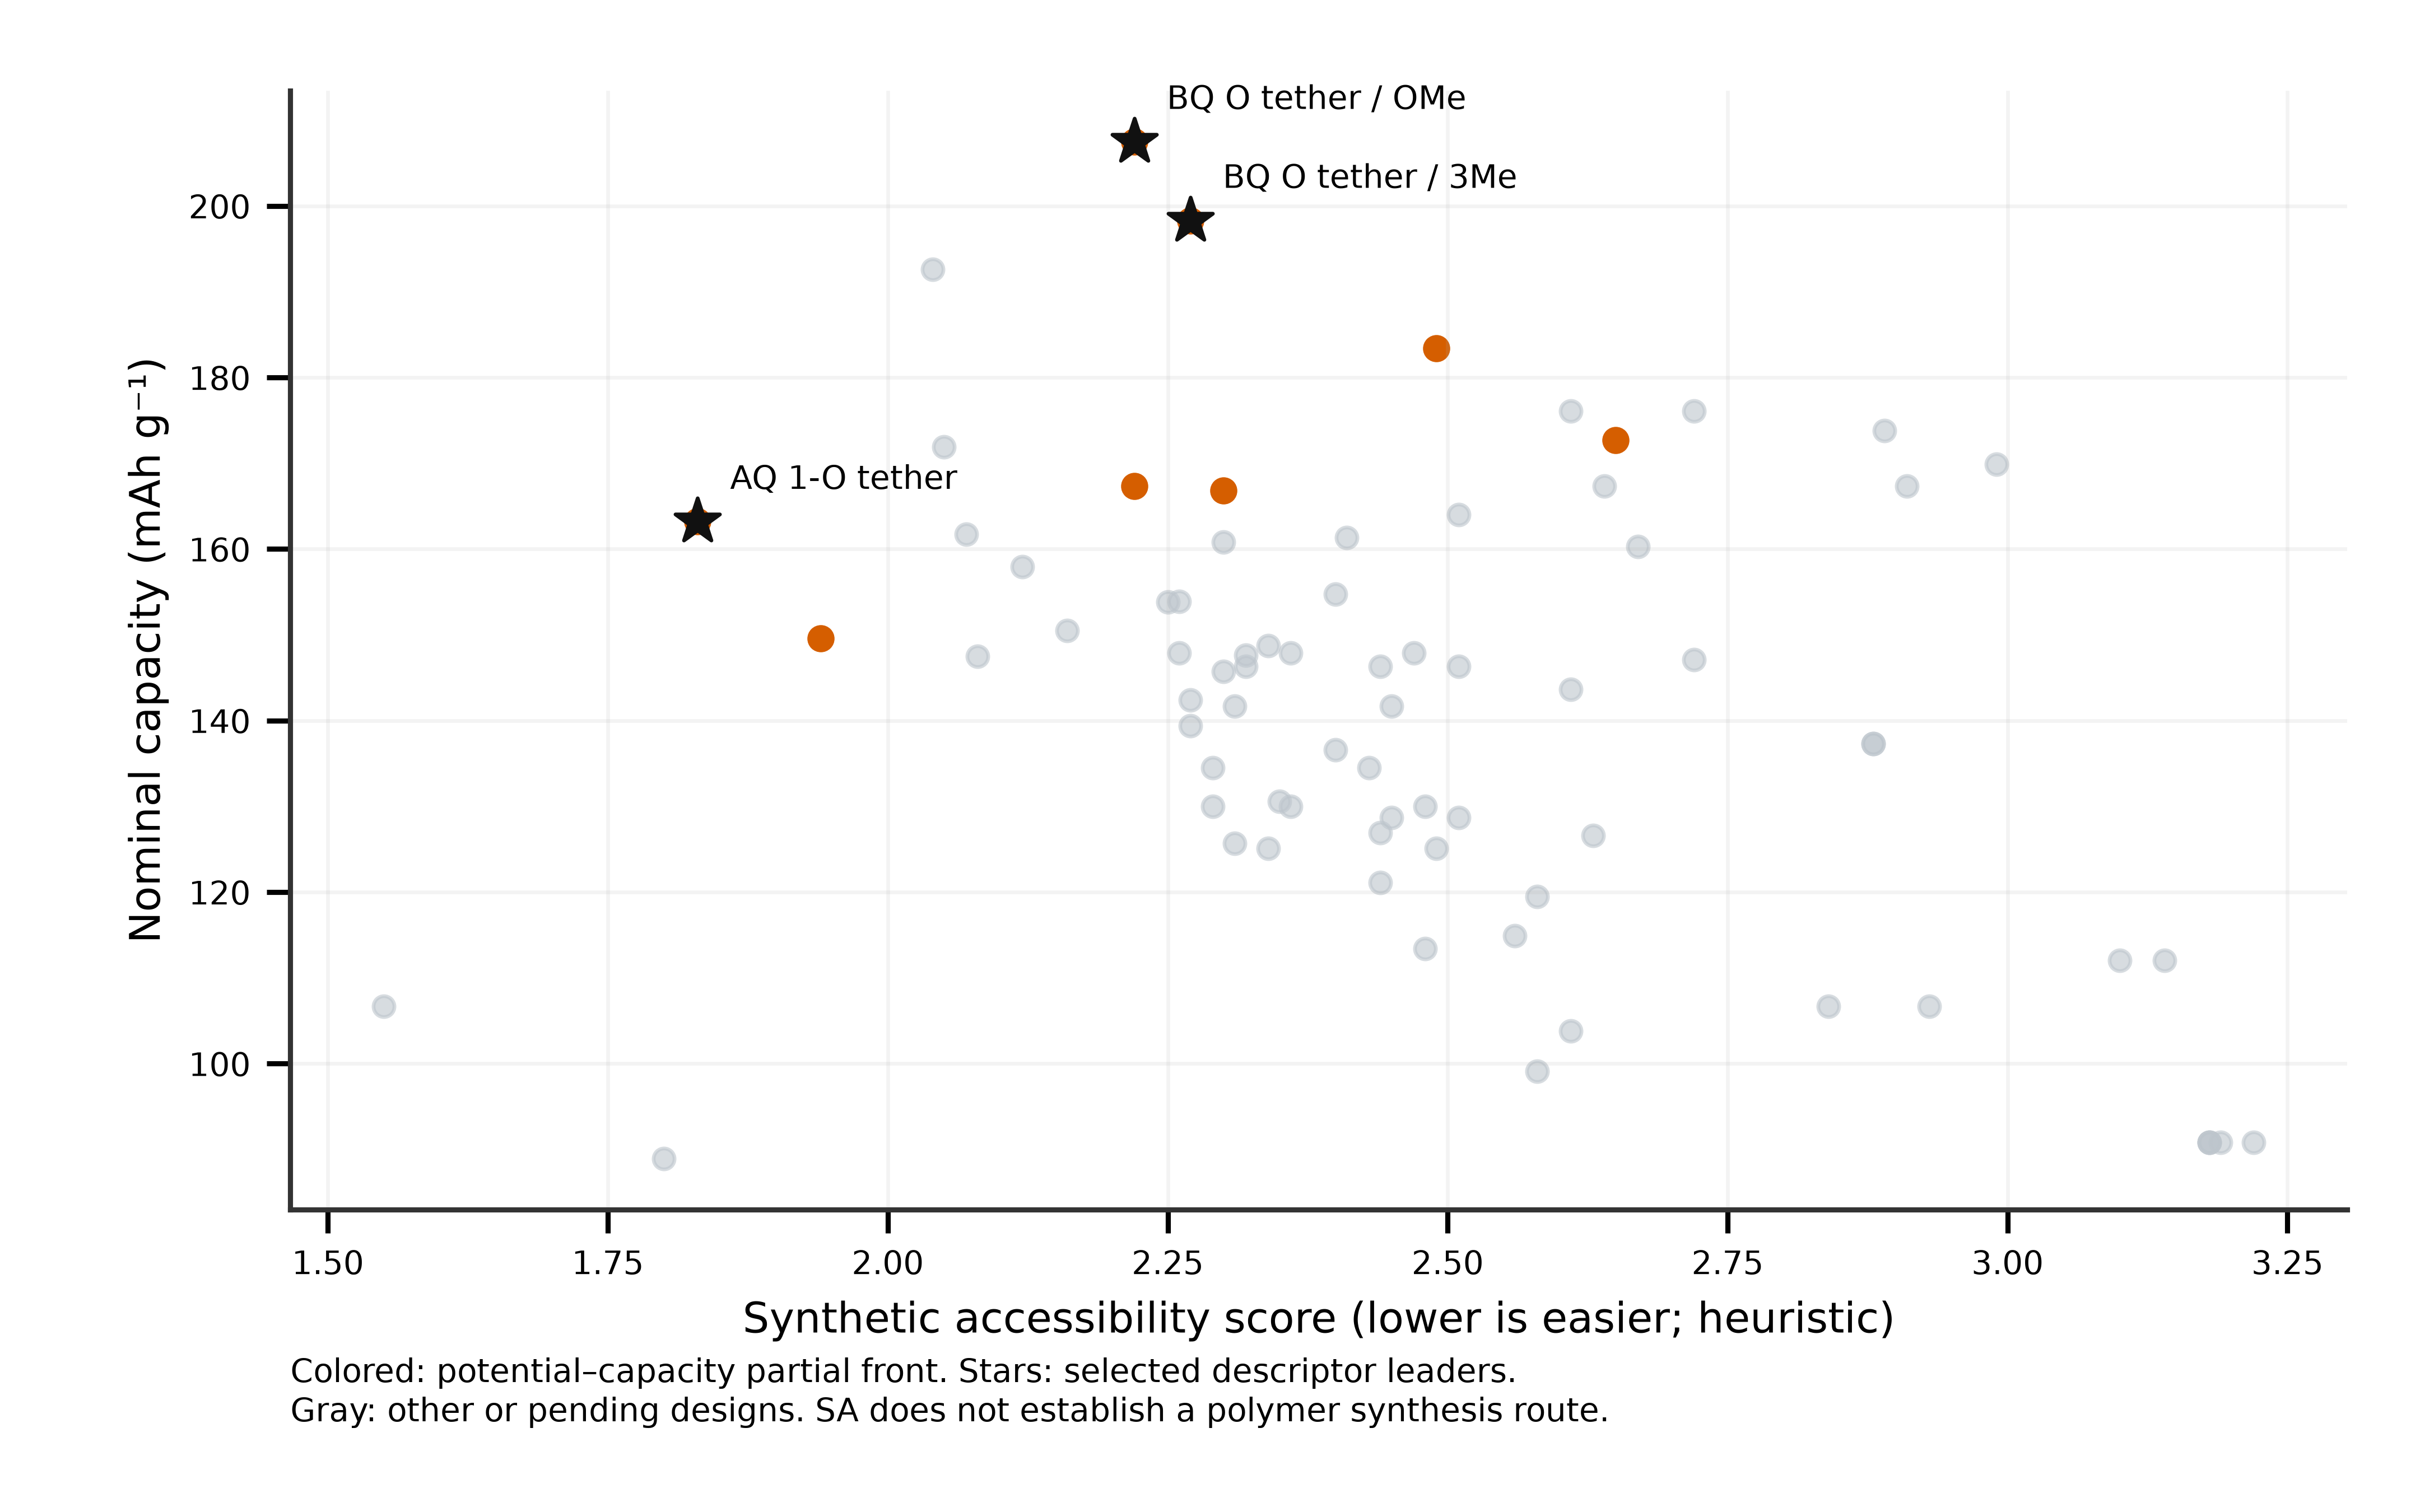
\includegraphics[width=.97\linewidth,height=.72\textheight,keepaspectratio]{../results/candidates/figures/synthesis_tradeoff.png}
\par\smallskip\raggedright\scriptsize SA is a heuristic annotation. The computed methylbenzyl caps lack the vinyl group required for monomer-first polymerization.
\vfill\tiny Audited model snapshot: 2026-10-19T12:22:05.478576-05:00.
\end{frame}
\begin{frame}{New candidate contrasts against matched controls}
\centering
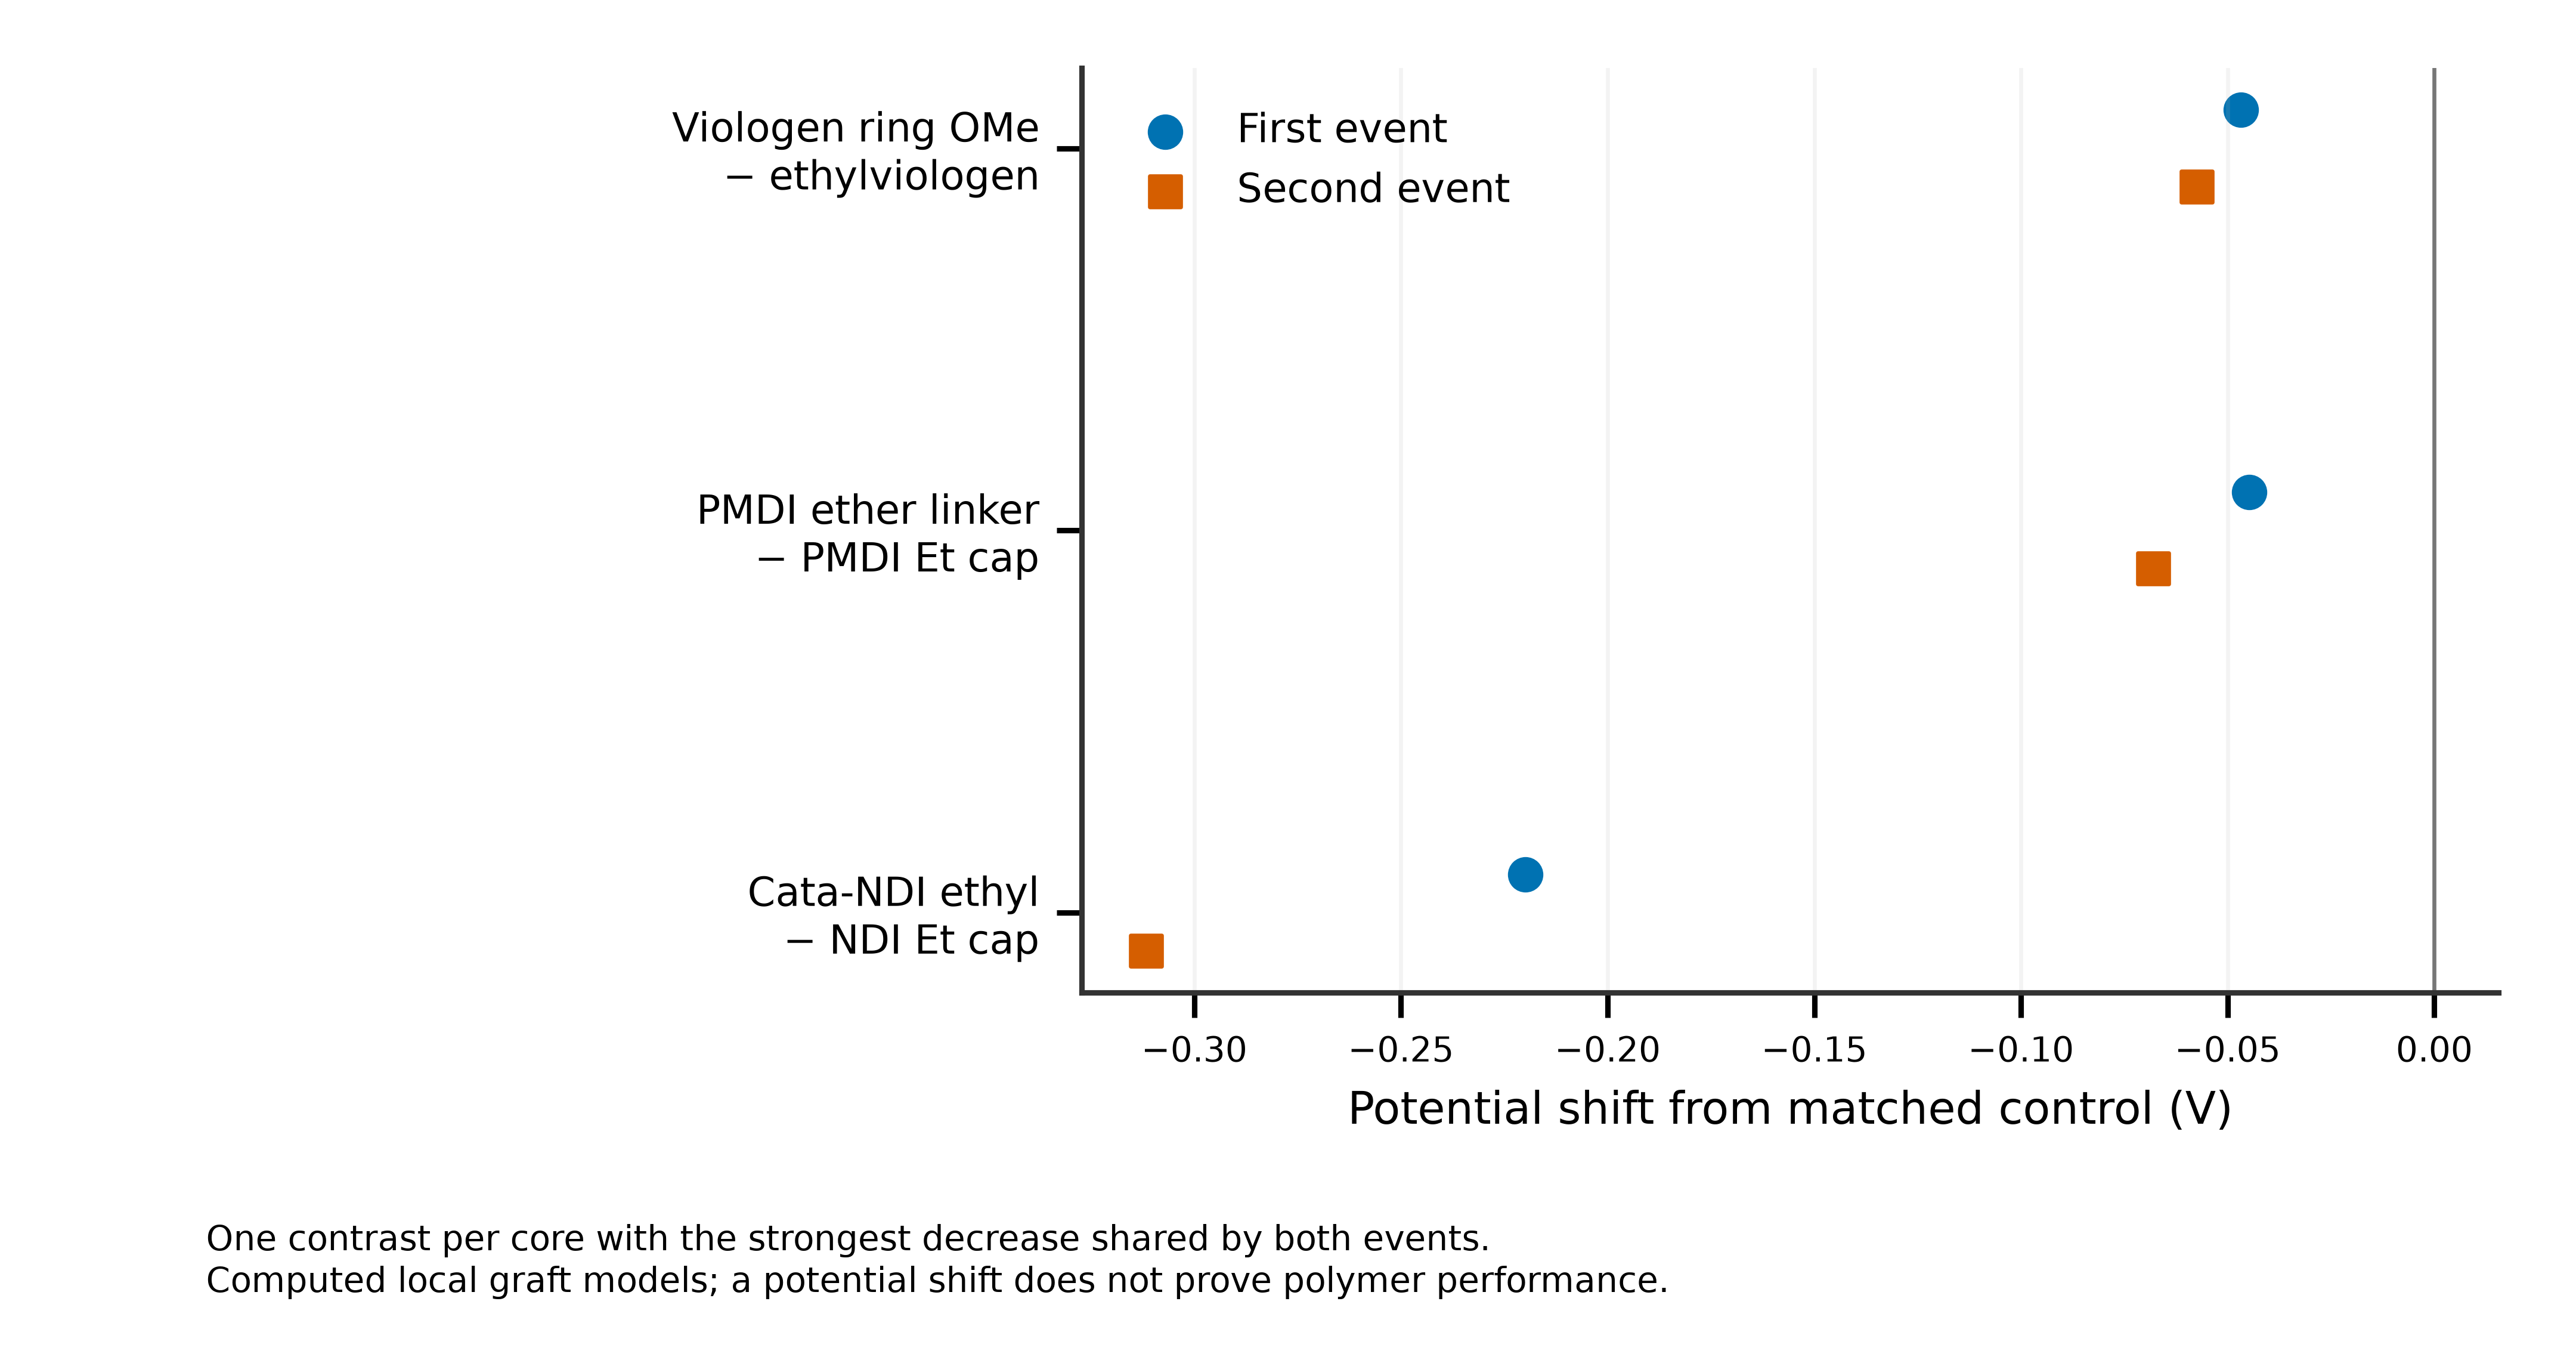
\includegraphics[width=.97\linewidth,height=.72\textheight,keepaspectratio]{../results/candidates/figures/new_candidate_shifts.png}
\par\smallskip\raggedright\scriptsize One contrast per core with the strongest potential decrease shared by both events. A shift does not establish polymer performance.
\vfill\tiny Audited model snapshot: 2026-10-19T12:22:05.478576-05:00.
\end{frame}
